\chapter{Noyau de l'application (Guillaume)}

	\section{Analyse}

		Structures de données et fonctionnalités
	
		-> Listes, sous-listes, tâches
		
	\section{Fonctionnalités}
	
		ghsdkglhsd
		
		


\chapter{Prototyping (Jerome)}

	\section{Storyboard}
		\begin{figure}[h!]
		   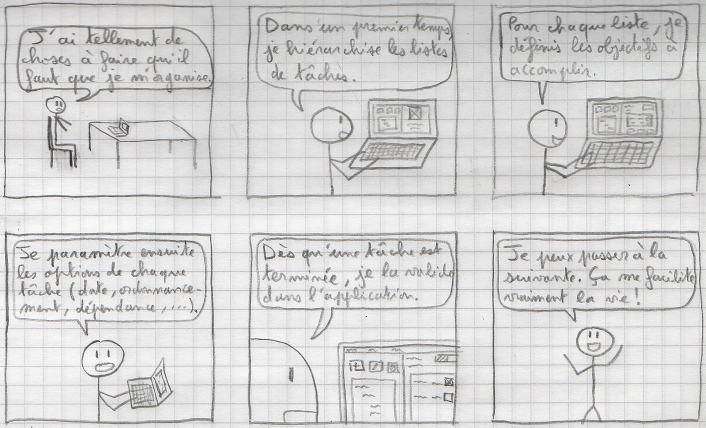
\includegraphics{img/stotyboard_ihm.png}
		   \caption{Storyboard de l'utilisation de l'application}
		\end{figure}
	
		La planche ci-dessus présente les différentes étapes d'utilisation basique du logiciel par un utilisateur lambda (son niveau de compétence n'entre pas ici en compte). Voici la liste des fonctionnalités évoquées et qui devront être présentes dans l'application finale :
		\begin{itemize}
			\item Création de listes imbriquées de tâches;
			\item Paramétrages possibles : dates relatives ou absolues, ordonnancement et dépendance des tâches;
			\item Validation des tâches et affichage de l'avancement;
			\item Sauvegarde en local des modifications effectuées.
		\end{itemize}
	
		Une fois le contexte d'utilisation cerné, il faut maintenant réaliser le prototype papier pour permettre
	
	\section{Prototype papier}
	Une \href{https://www.youtube.com/watch?v=xbLaZvgkzjQ}{vidéo sur Youtube} est accessible pour montrer le fonctionnement de l'interface du prototype papier. Le rendu vidéo est en deça de ce à quoi nous nous attendions mais nous n'avons pas eu les conditions optimales (matérielles et logicielles) de production.
	
	TODO
	

	\section{Scénarios d'utilisation}
		Plusieurs scénarios sont envisageables dans le cadre de notre application, en voici une liste non-exhaustive :
	
		\begin{itemize}
			\item C'est la première fois que l'utilisateur teste le logiciel, il le lance et commence de zéro. Il va dans un premier temps créer les listes puis créer les tâches associées. Il peut ensuite paramétrer les dates et les dépendances. A n'importe quel moment il va pouvoir sauvegarder les informations en format xml sous le nom qu'il souhaite, et ce même s'il existe par défaut une sauvegarde automatique silencieuse. Il ne lui reste plus qu'à valider les tâches pour prendre en compte son avancement global.
			\item L'utilisateur a déjà créé un fichier précédemment : il va pouvoir charger le fichier correspondant et continuer son travail là où il en était rendu. Dans le cas où certaines tâches ou listes ne sont plus d'actualité, il est possible de les modifier ou supprimer. Lorsque l'utilisateur va vouloir quitter l'application, un message va lui demander s'il souhaite conserver les modifications ou les annuler. 
		\end{itemize}
	
	
	\section{Évaluation du prototype}
		Pour avoir un point de vue extérieur, nous avons demandé à un étudiant (qui a souhaité gardé l'anonymat) de nous donner son avis sur le prototype papier. TODO 
		On a demandé à Péneau ce qu'il pensait de notre paper-prototype, il a dit OK et on a modifié 2-3 trucs :)
		


\chapter{IHM}
	
	\section{Présentation (Guillaume)}
		screens
		dire que y a des popup pour confirmer la suppression (pas faire de caca) ou pour signaler à l'utilisateur que son action n'est pas possible (modifier une tache alors que y en a pas)
	
	\section{Ergonomie (Jerome)}
		Toute la difficulté pour la réalisation de l'interface graphique d'une telle application est de permettre de proposer à l'utilisateur néophyte un rendu clair et intuitif tout en proposant des fonctionnalités plus avancées pour un {\oe}il plus expert. Pour réussir cela, nous avons listé les différentes fonctionnalités souhaitées par ces deux groupes d'utilisateurs et les moyens possibles pour y arriver.
		
		Pour cela, nous avons décider de proposer plusieurs moyens d'arriver aux mêmes fonctionnalités. Par exemple, pour la création de tâches on peut passer par le menu de l'application, le bouton (+) sur la partie droite de l'écran, le clic droit sur cette même partie ou bien le raccourcis clavier. De cette manière, l'utilisateur aura toujours une solution qui lui conviendra plus que les autres et qu'il considèrera comme plus intuitive.
		
		De plus, nous avons choisi de toujours afficher le même menu pour ne pas perdre l'utilisateur avec des \og modes \fg d'utilisation. Ainsi, l'utilisateur aura toujours les mêmes repères visuels. Cela est important, en particulier pour les débutants, qui ne peuvent pas se raccrocher à leur expérience avec d'autres logiciels similaires.\newline
		
		Pour rendre l'utilisation plus intuitive, nous avons aussi décidé d'intégrer des icônes colorées, explicites et facilement reconnaissables pour limiter la quantité de texte à l'écran. Pour cela, nous avons utilisé des images tirées de la bibliothèque du projet \emph{Gnome}\footnote{\href{https://commons.wikimedia.org/wiki/GNOME_Desktop_icons}{Icônes disponibles ici.}} et disponibles sous licence GNU General Public License version 2. Les avantages de ces icônes sont nombreux : gratuits, libres, ergonomiques et disponibles en de nombreuses tailles, \dots \newline
		
		Nous avons souhaité permettre à l'utilisateur de contrôler dans une certaine mesure la taille des panneaux, c'est pourquoi nous avons permis d'agrandir l'un ou l'autre des côtés de la vue avec un /emph{splitter} vertical pour une meilleure lisibilité.
		
		En plus de cela, nous affichons une petite aide lors du lancement du programme pour permettre une prise en main rapide et aisée. En effet, le panneau dédié aux liste de tâche est temporairement remplacé par un message de bienvenue qui avertit l'utilisateur sur le fonctionnement du logiciel.
		
		
	\section{Structure des widgets (Guillaume)}
		
		
	
\chapter{Limites de l'application (TOUS)}
	Une des limites de l'application est la variation du rendu de l'interface graphique en fonction des systèmes d'exploitation ou/et des gestionnaires de fenêtres utilisés. Ce problème étant inhérent à Qt, il est cependant possible de diminuer son impact en ajoutant \og -style=cleanlooks \fg dans les options de lancement du programme. Cela permet plusieurs choses : sur certains système l'interface est plus agréable à l'{\oe}il, les fenêtres de dialogues peuvent proposer des icônes claires pour les boutons \emph{Ok} et \emph{Annuler} et cela permet d'uniformiser un peu plus les rendus. De plus, certains éléments comme le splitter, qui permet de modifier la taille des panneaux, sont plus visibles et un peu plus gros. Cela rend l'interface de l'application plus intuitive et plus explicite.
	
	Cependant, nous n'avons pas essayé notre application sur d'autres systèmes d'exploitation, nous ne garantissons pas ni son bon fonctionnement, ni l'intégrité de l'interface graphique. En revanche, les tests sur les machines du CIE ont été concluants, comme il était demandé dans le sujet du TP.\\
	
	 Un autre problème de l'application est l'impossibilité de redimentionner la fenêtre principale. Cette limitation est dûe à la présence de bugs graphiques particulièrement gênants lorsque ce redimentionnement était possible. Puisque nous voulions nous préoccuper des principales fonctionnalités en priorité, nous avons abandonné celle-ci qui ne nous semblait pas incontournable. Si nous avions bénéficié de plus de temps, cela fait partie des changements que nous aurions pu apporter.\\
	
	
	


\chapter{Évaluations (TOUS)}
	
	Utilisateurs néophytes :
		Ma mère et ma soeur
		Ta mère
		
	Utilisateurs avancés :
		Pierre-Yves
		Leroux

